\documentclass[letter,11pt]{amsart}
\usepackage{amsmath,amsfonts,amssymb}
\usepackage{tikz}

\begin{document}

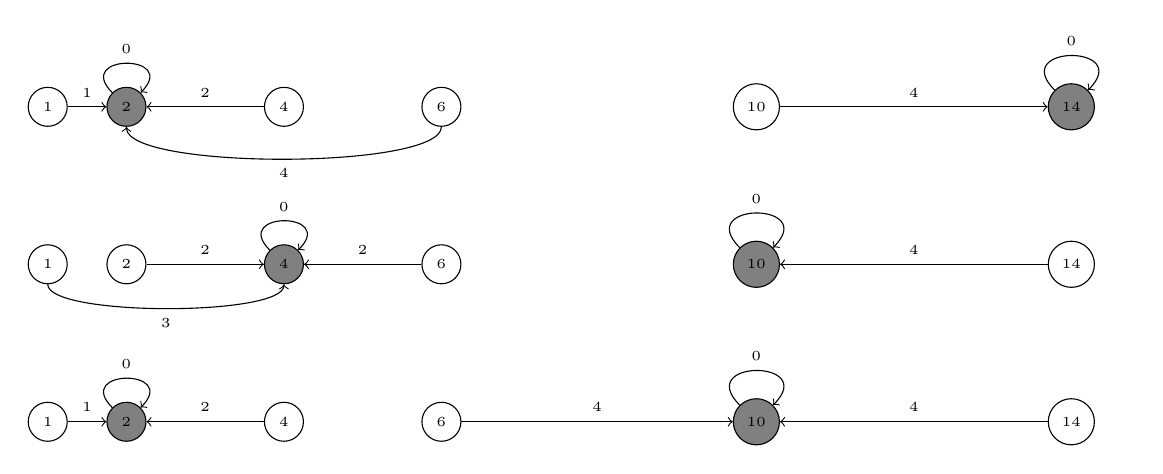
\begin{tikzpicture}[scale=1]

\def \margin {2} % margin in angles, depends on the radius


  \node[draw, circle] (A1) at (1,0) {\tiny $1$};
  \node[draw, circle, fill=gray] (A2) at (2,0) {\tiny $2$};
  \node[draw, circle] (A4) at (4,0) {\tiny $4$};
  \node[draw, circle](A6) at (6,0) {\tiny $6$};
  \node[draw, circle](A10) at (10,0) {\tiny $10$};
  \node[draw, circle, fill=gray](A14) at (14,0) {\tiny $14$};
  
  \path[->] (A1) edge node[above] {\tiny 1} (A2);
  \path[->] (A2) edge[out=135,in=45,looseness=5] node[above] {\tiny 0} (A2);
  \path[->] (A4) edge  node[above] {\tiny 2} (A2);
  \path[->] (A6) edge [out=270, in=270, ,looseness=0.35]  node[below] {\tiny 4} (A2);
 \path[->]  (A10) edge node[above] {\tiny 4} (A14);
 \path[->]  (A14) edge [out=135,in=45,looseness=5]   node[above] {\tiny 0} (A14);
 

 \node[draw, circle] (B1) at (1,-2) {\tiny $1$};
  \node[draw, circle] (B2) at (2,-2) {\tiny $2$};
  \node[draw, circle, fill=gray] (B4) at (4,-2) {\tiny $4$};
  \node[draw, circle](B6) at (6,-2) {\tiny $6$};
  \node[draw, circle, fill=gray](B10) at (10,-2) {\tiny $10$};
  \node[draw, circle](B14) at (14,-2) {\tiny $14$};
  
  \path[->] (B1) edge[out=270, in=270, ,looseness=0.35]  node[below] {\tiny 3} (B4);
  \path[->] (B2) edge node[above] {\tiny 2} (B4);
  \path[->] (B4) edge [out=135,in=45,looseness=5]   node[above] {\tiny 0} (B4);
  \path[->] (B6) edge  node[above] {\tiny 2} (B4);
 \path[->]  (B10) edge [out=135,in=45,looseness=5]  node[above] {\tiny 0} (B10);
 \path[->]  (B14) edge  node[above] {\tiny 4} (B10);


 \node[draw, circle] (C1) at (1,-4) {\tiny $1$};
  \node[draw, circle, fill=gray] (C2) at (2,-4) {\tiny $2$};
  \node[draw, circle] (C4) at (4,-4) {\tiny $4$};
  \node[draw, circle](C6) at (6,-4) {\tiny $6$};
  \node[draw, circle, fill=gray](C10) at (10,-4) {\tiny $10$};
  \node[draw, circle](C14) at (14,-4) {\tiny $14$};
  
  \path[->] (C1) edge node[above] {\tiny 1} (C2);
  \path[->] (C2) edge [out=135,in=45,looseness=5]  node[above] {\tiny 0} (C2);
  \path[->] (C4) edge  node[above] {\tiny 2} (C2);
  \path[->] (C6) edge  node[above] {\tiny 4} (C10);
 \path[->]  (C10) edge [out=135,in=45,looseness=5]  node[above] {\tiny 0} (C10);
 \path[->]  (C14) edge  node[above] {\tiny 4} (C10);
 
\end{tikzpicture}

\end{document}